\chapter{Parameters identification}
\label{chap:paramidentification}
\section{Steady state analysis}
\label{sec:steadystate}
Using the data of the file \emph{data\_steps.mat}, we analysed the step response
of the system by going to check the relationships between the stiffness of the 
springs. 
And estimating a new coefficient for the voltage-to-force.
The estimate of a new voltage-to-force coefficient is carried out using the 
equation \eqref{eq:matrixform}:
\begin{equation} 
\label{eq:voltage-force}
	[K] x = \begin{bmatrix}
 			g_{\text{v}}	\\
 			0 	\\
 			0
 		\end{bmatrix} \cdot v
\end{equation}
and therefore from \eqref{eq:voltage-force} it is possible to derive:
\begin{equation} \label{eq:voltageforce}
	g_{\text{v}} = [K] \begin{bmatrix}
	x_{1}\\
	x_{2}\\
	x_{3}
	\end{bmatrix}\frac{1}{v}
\end{equation}
Using the steady state value of the three output and the equation 
\eqref{eq:voltageforce} it is possible to evaluate the ratio of the stiffness 
of the springs with respect to  the nominal value of the third spring indicated 
with $k_3$, so it is possible to rewrite:
\begin{equation}
	\label{eq:gvestimate}
	k_3 \begin{bmatrix}
		x_1\\
		x_2\\
		x_3\\
	\end{bmatrix} = v \cdot
	\begin{bmatrix}
		g_{\text{v}} + g_{\text{v}} \cdot \frac{k_3}{k_1} + g_{\text{v}} \cdot 
		\frac{k_{3}}{k_{2}}\\
    		g_{\text{v}} + g_{\text{v}} \cdot \frac{k_{3}}{k_{2}}\\
    		g_{\text{v}}
    \end{bmatrix}
\end{equation}
\begin{figure}[htb]
	\centering
	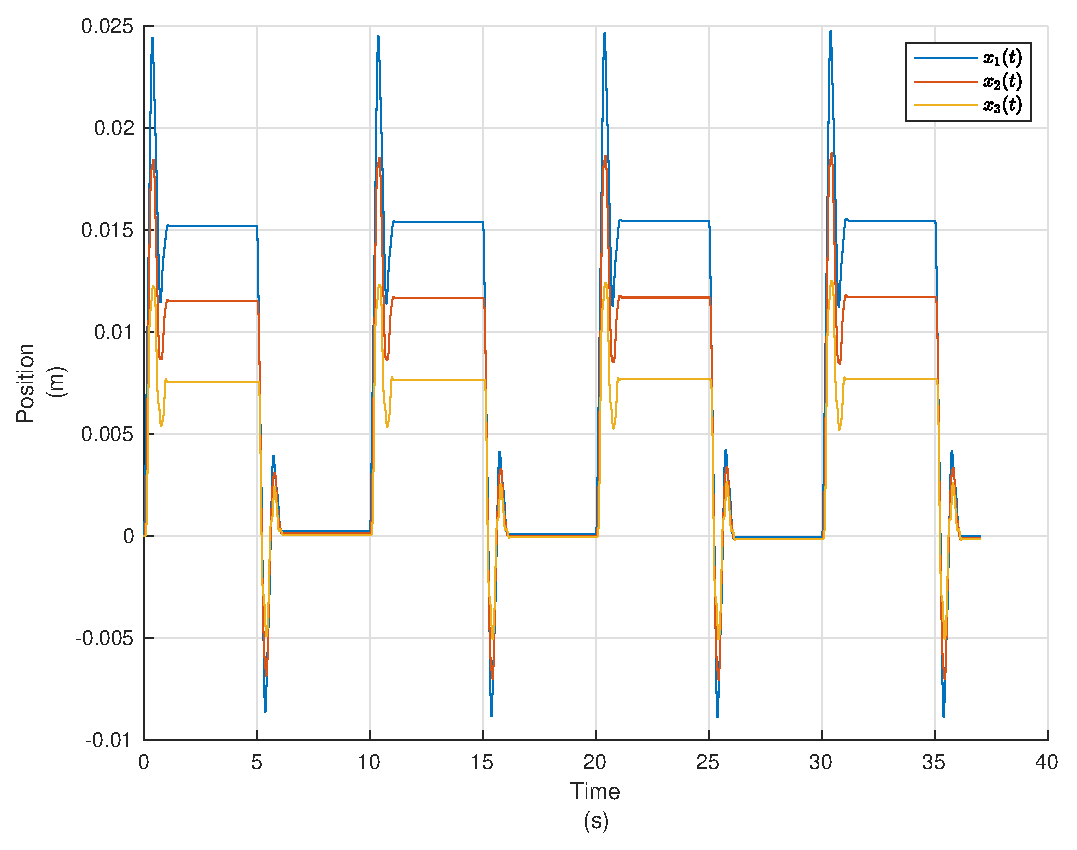
\includegraphics[width=0.75\textwidth]{steadystate}
	\caption{Steady state value pick}
	\label{fig:steadystate}
\end{figure}\linebreak
\noindent From the above equation \eqref{eq:gvestimate} we obtain the results: nominal 
and estimated ratios between the stiffness of the springs as well as the 
coefficient voltage-to-force.
The value of steady state response \(x_{i}\) are picked from the data directly 
in a point far from the transient, as shown in Figure \ref{fig:steadystate}.
To reduce the zero-mean noise an average with the previous \(400\) samples, 
i.e. a range between 2[\si{\second}] and 4[\si{\second}].
The table \ref{tab:error} shows values and it is possible to appreciate in the 
last column the error made on the estimate of these values, according to the 
formulation:
\begin{equation}
	\label{eq:ratioerror}
	\text{\textbf{err}} = 100\cdot\frac{\text{computed}}{\text{nominal}}
\end{equation}
%
\begin{table}[ht]
\centering
	\begin{tabular}{lrrr}
	\toprule
						& nominal & computed & error [\%] \\
 	\midrule
 		ratio $k_{3}/k_{1}$	& 0.50000 & 0.48935 &	2.17651 \\
		ratio $k_{3}/k_{2}$	& 0.50000 & 0.52086 & 	4.00560 \\
		gain ratio $g_{\text{v}}$ & 5.25000 & 6.04866 &  15.21248	\\
	\bottomrule
	\end{tabular}
	\caption{ratio between the stiffness constants and voltage-to-force coefficients}
	\label{tab:error}
\end{table}
%
\section{System identification}
\label{sec:sysidentification}
It is necessary to estimate the parameters of three \textsc{dof} system at simple 
identification, so that the impulse response is used to suppose that a model is 
based on a set of parameters, identifying the inputs as the initial force and 
conditions and the output of the system.
Thus comparing the system response measured with that predicted by the model.\\
Defined a model for the system: depends on a set of parameters $\theta$. 
Identify the input (strength and initial conditions) and output $(x(t))$ of the system. 
By giving the same input to the model and comparing the measured response $x(t)$ 
to that expected by the model $(x(t,\theta))$.
%
\begin{figure}[htb]
	\centering
	\resizebox{.50\linewidth}{!}{\begin{tikzpicture}
% help guide lines
%\draw[help lines] (0,0) grid [step = 5 mm](10,10);
%\foreach \x in {0,1,...,10}
%   \draw [help lines] (\x,0) node [below,%
%          font=\footnotesize] {$\x$} -- (\x,0);
%\foreach \y in {0,1,...,10}
%   \draw [help lines] (0,\y) node [left,%
%          font=\footnotesize] {$\y$} -- (0,\y);
%
% define model box
\newcommand{\modelbox}[2]{
	% input arrow  
	\coordinate (startarrow) at ({#1},{#2});
	\coordinate	(endarrow) at ($(startarrow)+(2.5,0)$);
	\draw [-stealth]($(startarrow) + (0,1 * 1)$) -- ($(endarrow)+(0,1* 1)$) node[above, midway] {$f(t)$};
	\draw [-stealth]($(startarrow) + (0,1 * 0)$) -- ($(endarrow)+(0,1* 0)$) node[above, midway, xshift=-0.65mm] {$\vec{x}_{0} \,, \dot{\vec{x}}_{0}$};
	% box
	% left low corner
	\coordinate (llcorner) at (2.5,-0.5);
	% right up corner
	\coordinate (rupcorner) at(6.5,1.5);
	\draw (llcorner) rectangle (rupcorner) node [midway]{dynamic system};
	% output arrow
	\coordinate (outputstartarrow) at (6.5,0.5);
	\coordinate	(outputendarrow) at (8.5,0.5);
	\draw [-stealth](outputstartarrow) -- (outputendarrow) node[above, midway] {$\vec{x}(t)$};
};
% 1 - plot the system model
\begin{scope}[yshift = 60mm]
   \modelbox{0}{0};  
\end{scope}
% 2 - plot second model and connection
\begin{scope}[yshift = 25mm]
   \modelbox{0}{0};
   \fill (1.75,1) circle (1.4pt);
   \fill (1,0) circle (1.4pt);
\end{scope}
% connect system model
   \draw (1.75,1) -- (1.75,3.5);
   \draw (1,2.5) -- (1,0);
% box model
\begin{scope}[xshift = 0mm]
   % input arrow  
	\coordinate (startarrow) at (1.75,1);
	\coordinate	(endarrow) at (2.5,1);
	\draw [-stealth](startarrow) -- (endarrow) node[below, midway] {$f(t)$};
	\draw [-stealth](1,0) -- (2.5,0) node[below, midway] {$\vec{x}_{0} \,, \dot{\vec{x}}_{0}$};
	% box
	% left low corner
	\coordinate (llcorner) at (2.5,-0.5);
	% right up corner
	\coordinate (rupcorner) at(6.5,1.5);
	\draw (llcorner) rectangle (rupcorner) node [midway]{model $\theta$};
	% output arrow
	\coordinate (outputstartarrow) at (6.5,0.5);
	\coordinate	(outputendarrow) at (8.5,0.5);
	\draw [-stealth](outputstartarrow) -- (outputendarrow) node[above, midway] {$\vec{x}(t)$};
\end{scope}
\end{tikzpicture}}
	\label{fig:systemmodel}
	\caption{System identification: real system and model}
\end{figure}
%
\\We define the residue as the difference between the two signals as in the 
equation \eqref{eq:residual}.
\begin{equation}
\label{eq:residual}
	\varepsilon(t,\theta) = x(t) - x(t,\theta)
\end{equation} 
The best choice for the set of parameter $\theta$ is the one that minimizes the 
residue integer (\ref{eq:residualinteger}) of the residue. 
\begin{equation}
\label{eq:residualinteger}
	\theta_{optim} = \text{argmin} \biggl( \int \varepsilon(t,\theta)^2 \, dt \biggr)
\end{equation} 
In this case, as the discrete signals with $N$ samples, the optimal value $N$ 
calculated as (\ref{eq:residualdiscrete}), this correspond to solving a least 
square problem.
\begin{equation}
\label{eq:residualdiscrete} 
\theta_{optim} = \text{argmin} \Biggl( \sum_{n=1}^{N} \varepsilon(t,\theta)^2 \Biggr)
\end{equation}
%
A linear model is adopted as described above, refer \ref{subsec:assumption}, 
assuming the stiffness matrix $[K]$ given.
Then quantifying the $[M]$ and $[C]$ parameters are used to minimize the problem.
Using the \emph{fmincon} algorithm, the problem is solved. In addition, the 
selected algorithm is required to specify the lower and upper search limits; 
as well as the first guess conditions from which the result is strictly dependent.
%
\subsection{Free damping case}
\label{subsec:freedamping}
Using the data of the file \emph{data\_impulse.mat} identify the seven parameters
previously identified in the model and described by the equation \eqref{eq:matrixform}. 
In this case, since the response to impulse force, two to approximation of the 
force estimation, will be analysed, the voltage-to-force coefficient will be 
estimated again.
The results of this optimization are shown in table \ref{tab:freedamping}.
\begin{table}[ht]
	\centering
	\begin{tabular}{SSSSSSS}
	\toprule
		\multicolumn{1}{c}%
			{$m_1$} & {$m_2$} & {$m_3$} & {$c_1$} &	 {$c_2$} & {$c_3$} & {$g_v$} \\
		\multicolumn{3}{c}{[\si{\kilo\gram}]}	&%
		\multicolumn{3}{c}{[\si{\newton\second\per\meter}]}	&%
		\multicolumn{1}{c}{[\si{\newton\per\volt}]}\\
	\midrule
          1.5712  & 1.5020  & 1.2018  &  2.7956 &  1.9978 & 2.1950  &  1.2096	\\
    \bottomrule
	\end{tabular}
	\caption{Optimizations results in free damping case}
	\label{tab:freedamping}
\end{table}
%
\begin{figure}[htb]
	\centering
	\subfloat[][\emph{mass vs displacement 1.}]
		{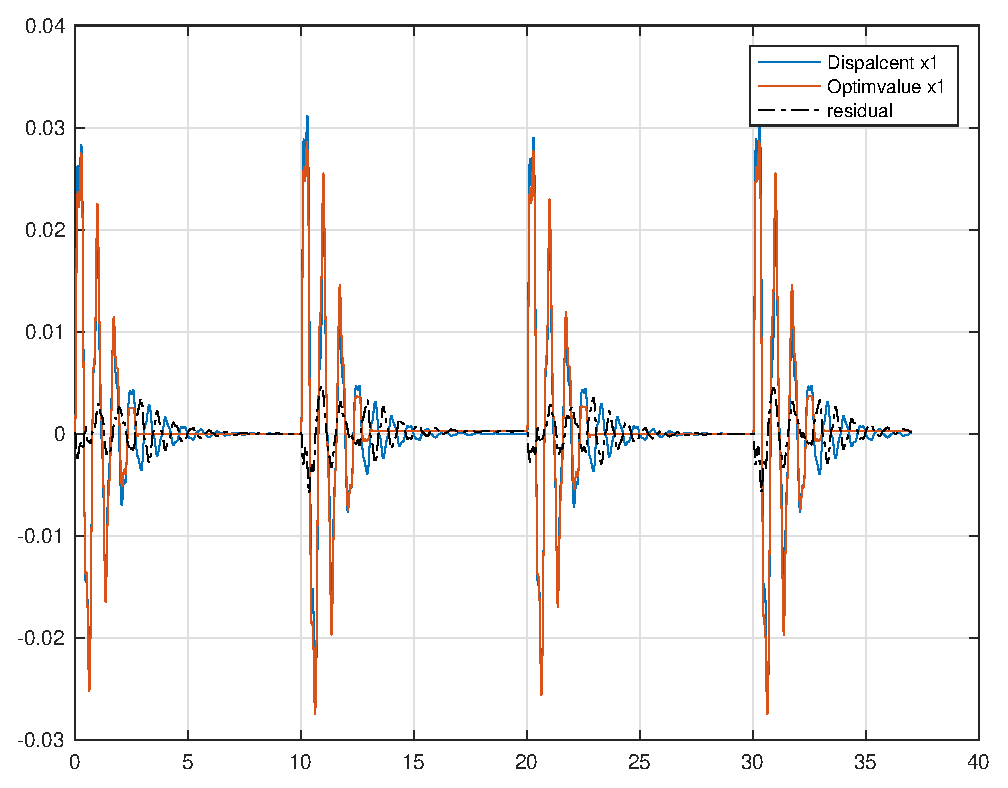
\includegraphics[width=0.75\textwidth]{residualfull1}}	\\
\end{figure}
%
\begin{figure}
	\ContinuedFloat
	\centering
	\subfloat[][\emph{mass vs displacement 2.}]
		{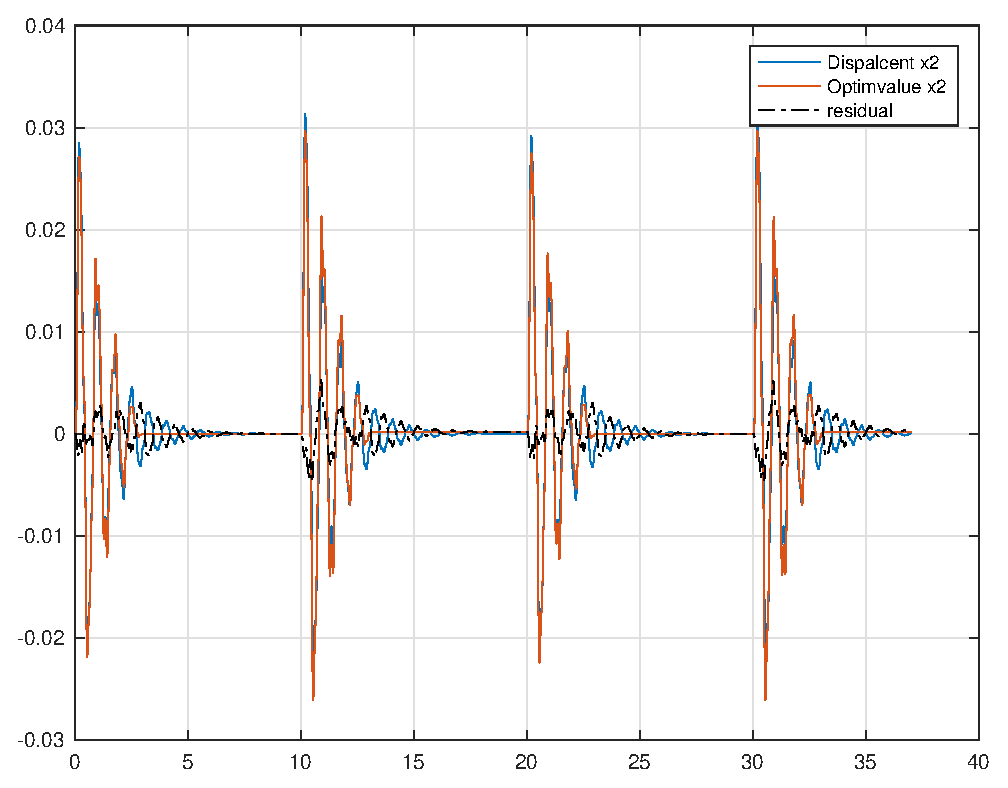
\includegraphics[width=0.75\textwidth]{residualfull2}}	\\
	\subfloat[][\emph{mass vs displacement 3.}]
		{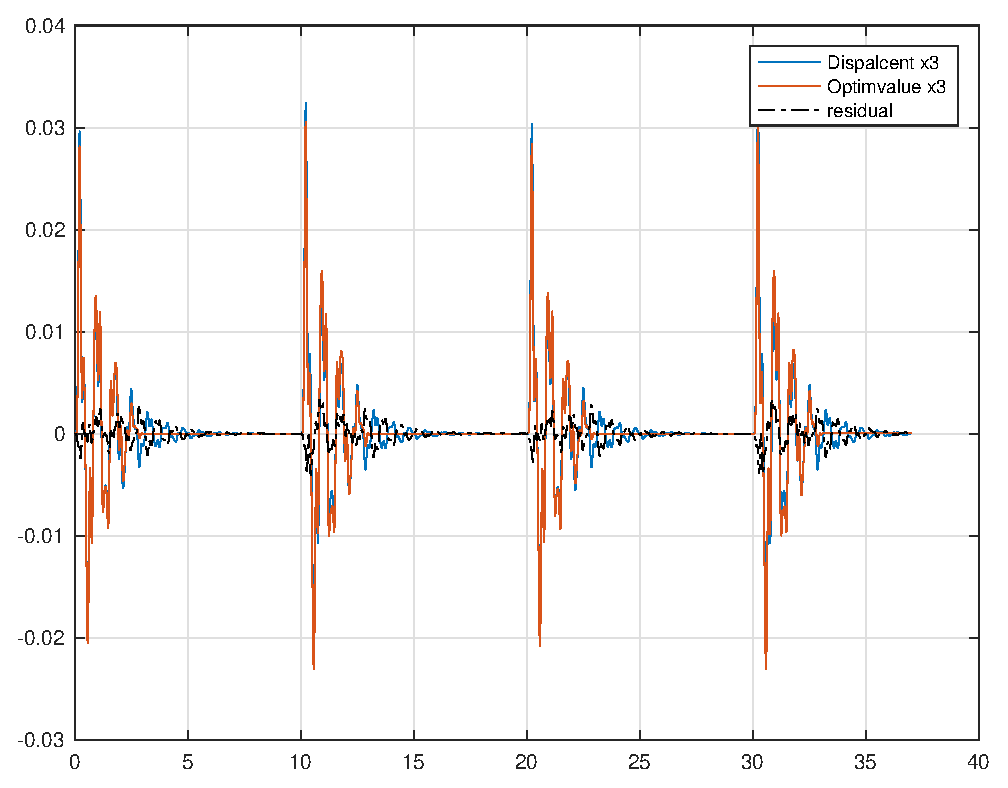
\includegraphics[width=0.75\textwidth]{residualfull3}}
	\caption{Comparison between the response of the model and the response of the 
	system free damping case}
	\label{fig:freedampingcase}
\end{figure}
%
\newpage
\subsection{Proportional damping case}
\label{subsec:proportionaldamping}
In this case, the procedure used to solve the problem of free damping to get 
used parameters, thus changing some conditions.
We define damping through the equation (\ref{eq:proportionaldamping}) where it 
is possible to observe that this depends on the linear combination of the mass 
matrix multiply by constant and the stiffness matrix multiply by the another 
constant.
Then the search limits and first guess will be changed to search the mass 
values and the unknown constants.
The interesting property of this representation is the ability to perform modal 
decomposition on the system.
\begin{equation}
\label{eq:proportionaldamping}
	[C] = \alpha \cdot [M] + \beta \cdot [K]
\end{equation}
The optimization results are available in the table \ref{tab:proportionaldamping}.
%
\begin{table}[htb]
	\centering
	\begin{tabular}{SSSSSS}
	\toprule
	\multicolumn{1}{c}%
			{$m_1$} & {$m_2$} & {$m_3$} & {$g_v$} &	 {$\alpha$} & {$\beta$} \\
	\multicolumn{3}{c}{[\si{\kilo\gram}]}	& %
	\multicolumn{1}{c}{[\si{\newton\per\volt}]} & %
	\multicolumn{2}{c}{[\si{\newton\second\per\meter}]} \\
	\midrule
       			1.5761   &  1.4970  & 1.1996  &  1.2094 &  1.6209   &  0.0001	\\
    \bottomrule
	\end{tabular}
	\caption{Optimizations results in proportional damping case}
	\label{tab:proportionaldamping}
\end{table}
%
\begin{figure}[htb]
\centering
	\subfloat[][\emph{mass vs displacement 1.}]
		{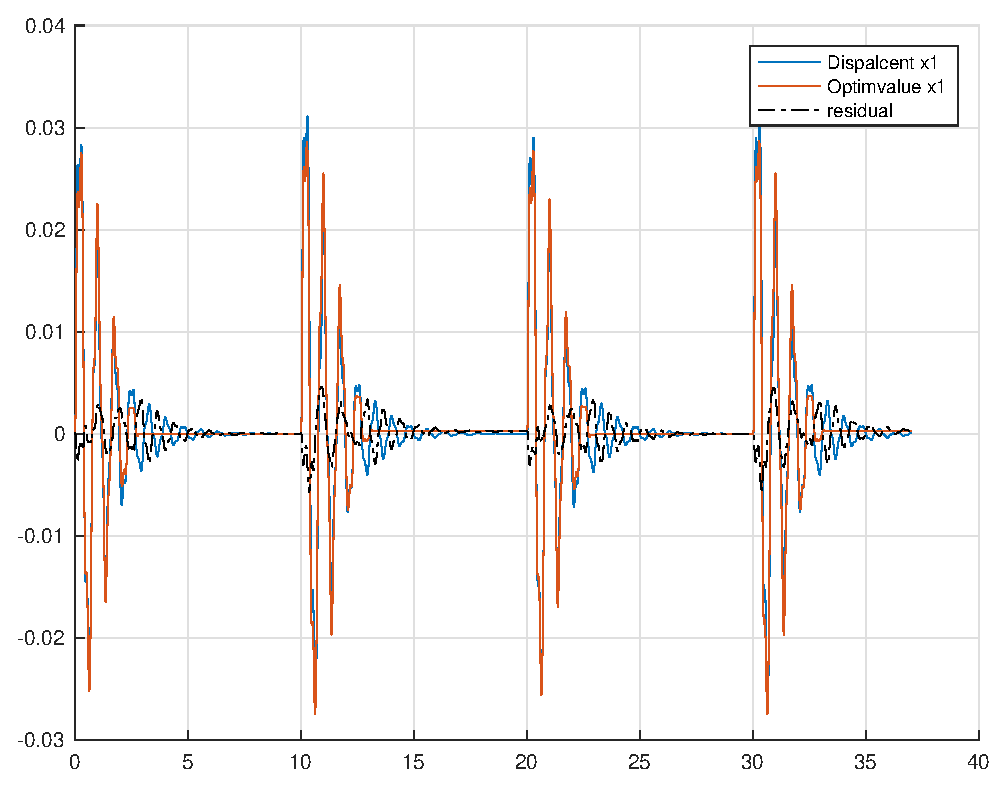
\includegraphics[width=0.75\textwidth]{residualpropdamp1}}	\\
\end{figure}
%
\begin{figure}
	\ContinuedFloat
	\centering	
	\subfloat[][\emph{mass vs displacement 2.}]
		{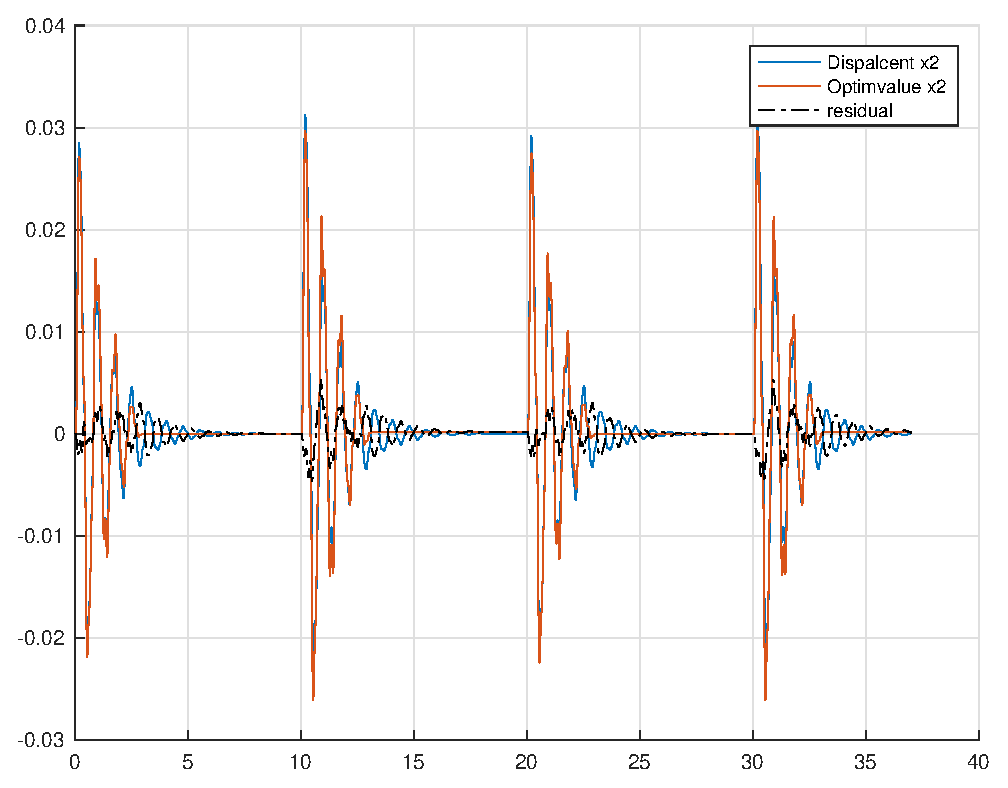
\includegraphics[width=0.75\textwidth]{residualpropdamp2}}	\\
	\subfloat[][\emph{mass vs displacement 3.}]
		{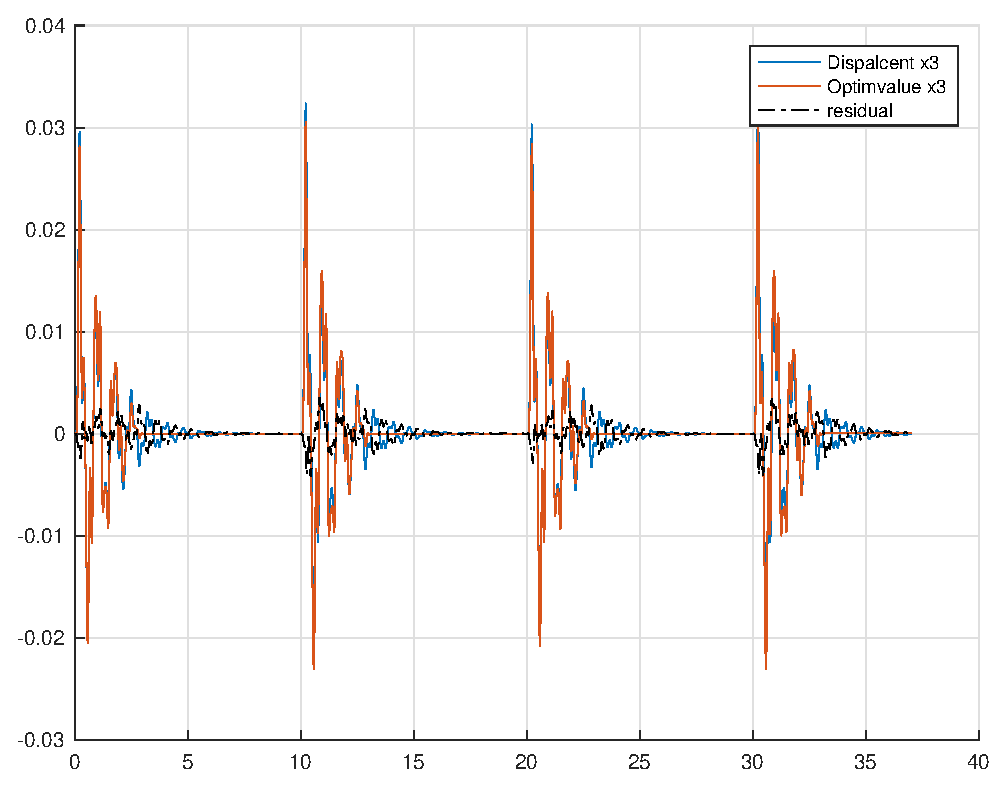
\includegraphics[width=0.75\textwidth]{residualpropdamp3}}	
	\caption{Comparison between the response of the model and the response of the system proportional damping case}
	\label{fig:proportionaldamping}
\end{figure}

Using modal superimposed method to compute the damping matrix \([C]\) requires 
that is orthogonal compared to natural mode, thus to satisfy this condition 
\([C]\) must expressed as seen in eq. \eqref{eq:proportionaldamping}.
The construction of the dynamic matrix of a system depends on the 
determination experimental of its dynamic response.
It is possible to use two different approaches:
\begin{itemize}
\item Considering a system one \textsc{dof} in case of damped oscillating 
motion and knowing his response given by equation
\(x(t) = x_{0} e^{-\zeta\omega_{n}t}sin(\omega_dt+\phi_0)\) it is possible excite 
selective of a single natural frequency and study of the free response. 
Consequently, the system will be excited according to the modal shape 
of interest and determining the value of \(\zeta_{k}\) by using logarithmic 
decrement as reported 
in \eqref{eq:log_decrement}.
\begin{equation}
\label{eq:log_decrement}
\delta = ln\frac{x(t+\tau)}{x(t)} = \frac{2\pi\zeta_{k}}{\sqrt{1-\zeta_{k}^2}}
\end{equation}
Knowing the others parameters it is possible compute the damping for the system. 
Then repeating the sequence above described is possible to determine the remainder
 parameters. 
\item Using Forced oscillation with spectrum analysis, by this way we obtain 
the spectrum that can be analysed by the equation:
\begin{equation}
\label{eq:analysis_spectrum}
\frac{X_{0}}{\frac{F_{0}}{k}} = \frac{1}{2\zeta\sqrt{1-\zeta^2_{k}}} \cong \frac{1}{2\zeta_{k}}
\end{equation}
Where the peak corresponds to resonance conditions and their amplitude is 
expressed by the term \(\frac{1}{2\zeta_{k}}\).
\end{itemize}
This is an approximation because in reality the amplitude of the oscillations 
at a given frequency is given by the superposition of all the modes of the 
system. This approach provides a reasonable approximation of \(\zeta_{k}\) only 
if the modes are sufficiently spaced.\\
The matrix of the proportional damping obtained is shown:
\begin{equation}
\label{eq:c-matrix}
	[C] =
	\begin{bmatrix*}[r]
		 2.64026		&	-0.08550		 & 	 0.00000 	\\
		-0.08550 	&	 2.59748		 &	-0.08550		\\
		 0.00000 	&	-0.08550		 &	 2.07270		\\
	\end{bmatrix*}
\end{equation}
\\In conclusion highlighting the \(\alpha\) term with respect to a given frequency, 
a damping behaviour is observed that is excellent to filter low frequency 
oscillations (high amplitude).
Instead, observing of  \(\beta\) term, damping stiffness, has a much lower 
value, seen in table \ref{tab:proportionaldamping}. 
Generally, \(\beta\) behaviour shows the ability to filter high frequency 
oscillations (small amplitude).
Last but not least it is possible to express the damping ratio as:
\begin{equation}
\label{eq:dampingratio}
\zeta = \frac{\alpha + \beta \omega^2}{2\omega}
\end{equation}
%
\subsection{Comparison}
\label{subsec:comparison}
After fitting data with a model, you should evaluate the goodness of fit. 
The goodness of fit is calculated using the normalized root mean square error 
as the cost function.
In table \ref{tab:goodoffit} are available the percentages the measured output.
This method to assess goodness of fit for both linear and non linear parametric 
fits.
As is common in statistical literature, the term goodness of fit is used here 
in sense: ``good fit" might be a model where the data could reasonably have 
come from, given the assumptions of least-squares fitting.
\begin{table}[ht]
\centering
\begin{tabular}{lccc}
	\toprule
		 & $x_1$ [\%] & $x_2$ [\%] & $x_3$ [\%]\\
	\midrule
	% free damping result
	free damping case & 81.36 & 81.17 & 81.71 \\
	% proportianl damping result
	proportional damping case & 81.36 & 81.17 & 81.56 \\
	\bottomrule
\end{tabular}
\caption{Result \emph{goodness of fit} measured output}
\label{tab:goodoffit}
\end{table}
%
\subsection{Multiple single DOF system case}
Alternatively, the system can be studied by breaking it down into simpler 
systems to a single degree of freedom. 
It is necessary to make simplifying hypotheses:
\begin{itemize}
\item each system is considered in equilibrium position;
\item known masses;
\item the dampers are placed in parallel and then summarized below:
\begin{equation}
\label{eq:eq_damp_1_dof}
\begin{cases}
c_1^{\text{\tiny 1-\textsc{dof}}} &= c_1\\
c_2^{\text{\tiny 1-\textsc{dof}}} &= c_1 + c_2\\
c_3^{\text{\tiny 1-\textsc{dof}}} &= c_1 + c_2 + c_3\\
\end{cases}
\end{equation}
\end{itemize}
In figures a possible configuration is shown.
\begin{figure}[htb]
	\centering
	\subfloat[][\emph{first system}]
		{\resizebox{0.45\linewidth}{!}{\begin{tikzpicture}
%\draw[help lines] (0,0) grid [step = 5 mm](15,3.5);
%\foreach \x in {0,1,...,15}
%   \draw [help lines] (\x,0) node [below,%
%          font=\footnotesize] {$\x$} -- (\x,0);
%\foreach \y in {0,1,...,3.5}
%   \draw [help lines] (0,\y) node [left,%
%          font=\footnotesize] {$\y$} -- (0,\y);

% Define style for spring
\tikzstyle{springshape}=[decoration={aspect=0.6, segment length=1.5mm, amplitude=1mm, coil}, decorate];
\newcommand{\spring}[3]{%
	% pass 3 arguments:
	% arg1: #1 coordinate x; arg2:  #2 coordiante y; arg3: #3 number of componets
	\coordinate (attachleftside) at ({#1},{#2});
	\coordinate (startspring) at ($(attachleftside) + (0.25,0)$);
	\coordinate	(endspring) at ($(startspring) + (2,0)$);
	\coordinate	(attachrightside) at ($(endspring) + (0.25,0)$);
	\draw (attachleftside) -- (startspring);
	\draw [springshape] (startspring) -- (endspring) node[draw=none,pos=0.5, above=0.5em] (){$k_{#3}$};
	\draw (endspring) -- (attachrightside);
}

% Define style for dampers
\tikzstyle{dampshape}=[decoration={markings, mark connection node=dmp,
  mark=at position 0.5 with
  {
    \node (dmp) [inner sep=0pt,transform shape,rotate=-90,minimum width=15pt,minimum height=3pt,draw=none] {};
    \draw  ($(dmp.north east)+(2pt,0)$) -- (dmp.south east) -- (dmp.south west) -- ($(dmp.north west)+(2pt,0)$);
    \draw ($(dmp.north)+(0,-5pt)$) -- ($(dmp.north)+(0,5pt)$);
  }
}, decorate]
\newcommand{\dampers}[3]{%
	% pass 3 arguments:
	% arg1: #1 coordinate x; arg2: #2 coordiante y; arg3: #3 number of componets
	\coordinate (attachleftside) at ({#1},{#2});
	\coordinate (startdamp) at ($(attachleftside) + (0.25,0)$);
	\coordinate	(enddamp) at ($(startdamp) + (2,0)$);
	\coordinate	(attachrightside) at ($(enddamp) + (0.25,0)$);
	\draw (attachleftside) -- (startdamp);
	\draw [{dampshape}] (startdamp) -- (enddamp) node[draw=none,pos=1, above] (){$c_{#3}^{\text{\tiny 1-\textsc{dof}}}$};
	\draw (enddamp) -- (attachrightside);
}

% Define ground
\tikzstyle{ground}=[fill,pattern=north east lines,draw=none,minimum width=2cm,minimum height=0.3cm, rotate=90];
\tikzstyle{groundc}=[fill,pattern=north east lines,draw=none,minimum width=10mm,minimum height=0.2cm, rotate=90];
\begin{scope}[xshift=-3cm]
	\draw  (0,2.5) circle (2);
	\node [draw=none, anchor = north west] at (2,2.5) {$J_{0}$};
	\draw  (-2,0) rectangle (2,0.5);
	\draw[ultra thick] (2,0.25) -- (3,0.25);
	\draw [thick, red](1,-0.35)--(1,-0.65);
	\draw [-stealth, thick, red] (1,-0.5) -- (2,-0.5);
	\node [draw=none, anchor = north west] at (2,-0.5) {$F$};
\end{scope}
% generate plot
\begin{scope}[xshift=0cm]
	\draw (0,0) rectangle (2,1) node[draw=none,pos=0.5] () {$m_{1}$};
	\spring{2}{0.5}{1};
	\dampers{1}{2}{1};
	\draw [thin] (4.5,1.5) -- (4.5,2.5);
	\draw [thin] (3.5,2) -- (4.5,2);
	\node [groundc,anchor=north]  at (4.5,2){};
	\draw [thick] (1,1) -- (1,2);
	\draw [thick, gray](1,-0.35)--(1,-0.65);
	\draw [-stealth, thick, gray] (1,-0.5) -- (2,-0.5);
	\node [draw=none, anchor = north west] at (2,-0.5) {$x_1$};
	\node [ground,anchor=north]  at (4.5,0.5){};
	\draw [thin](4.5,1.5)--(4.5, -0.5);
\end{scope}
\end{tikzpicture}
}} \\
		\subfloat[][\emph{second system}]
		{\resizebox{0.7\linewidth}{!}{\begin{tikzpicture}
%\draw[help lines] (0,0) grid [step = 5 mm](15,3.5);
%\foreach \x in {0,1,...,15}
%   \draw [help lines] (\x,0) node [below,%
%          font=\footnotesize] {$\x$} -- (\x,0);
%\foreach \y in {0,1,...,3.5}
%   \draw [help lines] (0,\y) node [left,%
%          font=\footnotesize] {$\y$} -- (0,\y);

% Define style for spring
\tikzstyle{springshape}=[decoration={aspect=0.6, segment length=1.5mm, amplitude=1mm, coil}, decorate];
\newcommand{\spring}[3]{%
	% pass 3 arguments:
	% arg1: #1 coordinate x; arg2:  #2 coordiante y; arg3: #3 number of componets
	\coordinate (attachleftside) at ({#1},{#2});
	\coordinate (startspring) at ($(attachleftside) + (0.25,0)$);
	\coordinate	(endspring) at ($(startspring) + (2,0)$);
	\coordinate	(attachrightside) at ($(endspring) + (0.25,0)$);
	\draw (attachleftside) -- (startspring);
	\draw [springshape] (startspring) -- (endspring) node[draw=none,pos=0.5, above=0.5em] (){$k_{#3}$};
	\draw (endspring) -- (attachrightside);
}

% Define style for dampers
\tikzstyle{dampshape}=[decoration={markings, mark connection node=dmp,
  mark=at position 0.5 with
  {
    \node (dmp) [inner sep=0pt,transform shape,rotate=-90,minimum width=15pt,minimum height=3pt,draw=none] {};
    \draw  ($(dmp.north east)+(2pt,0)$) -- (dmp.south east) -- (dmp.south west) -- ($(dmp.north west)+(2pt,0)$);
    \draw ($(dmp.north)+(0,-5pt)$) -- ($(dmp.north)+(0,5pt)$);
  }
}, decorate]
\newcommand{\dampers}[3]{%
	% pass 3 arguments:
	% arg1: #1 coordinate x; arg2: #2 coordiante y; arg3: #3 number of componets
	\coordinate (attachleftside) at ({#1},{#2});
	\coordinate (startdamp) at ($(attachleftside) + (0.25,0)$);
	\coordinate	(enddamp) at ($(startdamp) + (2,0)$);
	\coordinate	(attachrightside) at ($(enddamp) + (0.25,0)$);
	\draw (attachleftside) -- (startdamp);
	\draw [{dampshape}] (startdamp) -- (enddamp) node[draw=none,pos=1, above] (){$c_{#3}^{\text{\tiny 1-\textsc{dof}}}$};
	\draw (enddamp) -- (attachrightside);
}

% Define ground
\tikzstyle{ground}=[fill,pattern=north east lines,draw=none,minimum width=2cm,minimum height=0.3cm, rotate=90];
\tikzstyle{groundc}=[fill,pattern=north east lines,draw=none,minimum width=10mm,minimum height=0.2cm, rotate=90];
\begin{scope}[xshift=-3cm]
	\draw  (0,2.5) circle (2);
	\node [draw=none, anchor = north west] at (2,2.5) {$J_{0}$};
	\draw  (-2,0) rectangle (2,0.5);
	\draw[ultra thick] (2,0.25) -- (3,0.25);
	\draw [thick, red](1,-0.35)--(1,-0.65);
	\draw [-stealth, thick, red] (1,-0.5) -- (2,-0.5);
	\node [draw=none, anchor = north west] at (2,-0.5) {$F$};
\end{scope}
% generate plot
\begin{scope}[xshift=0cm]
	\draw (0,0) rectangle (2,1) node[draw=none,pos=0.5] () {$m_{1}$};
	\draw (2,0.5)--(4.5,0.5);
\end{scope}
\begin{scope}[xshift=4.5cm]
	\draw (0,0) rectangle (2,1) node[draw=none,pos=0.5] () {$m_{2}$};
	\spring{2}{0.5}{2};
	\dampers{1}{2}{2};
	\draw [thin] (4.5,1.5) -- (4.5,2.5);
	\draw [thin] (3.5,2) -- (4.5,2);
	\node [groundc,anchor=north]  at (4.5,2){};
	\draw [thick] (1,1) -- (1,2);
	\draw [thick, gray](1,-0.35)--(1,-0.65);
	\draw [-stealth, thick, gray] (1,-0.5) -- (2,-0.5);
	\node [draw=none, anchor = north west] at (2,-0.5) {$x_2$};
	\node [ground,anchor=north]  at (4.5,0.5){};
	\draw [thin](4.5,1.5)--(4.5, -0.5);
\end{scope}
\end{tikzpicture}
}}	\\
		\subfloat[][\emph{third system}]
		{\resizebox{0.9\linewidth}{!}{\begin{tikzpicture}
%\draw[help lines] (0,0) grid [step = 5 mm](15,3.5);
%\foreach \x in {0,1,...,15}
%   \draw [help lines] (\x,0) node [below,%
%          font=\footnotesize] {$\x$} -- (\x,0);
%\foreach \y in {0,1,...,3.5}
%   \draw [help lines] (0,\y) node [left,%
%          font=\footnotesize] {$\y$} -- (0,\y);

% Define style for spring
\tikzstyle{springshape}=[decoration={aspect=0.6, segment length=1.5mm, amplitude=1mm, coil}, decorate];
\newcommand{\spring}[3]{%
	% pass 3 arguments:
	% arg1: #1 coordinate x; arg2:  #2 coordiante y; arg3: #3 number of componets
	\coordinate (attachleftside) at ({#1},{#2});
	\coordinate (startspring) at ($(attachleftside) + (0.25,0)$);
	\coordinate	(endspring) at ($(startspring) + (2,0)$);
	\coordinate	(attachrightside) at ($(endspring) + (0.25,0)$);
	\draw (attachleftside) -- (startspring);
	\draw [springshape] (startspring) -- (endspring) node[draw=none,pos=0.5, above=0.5em] (){$k_{#3}$};
	\draw (endspring) -- (attachrightside);
}

% Define style for dampers
\tikzstyle{dampshape}=[decoration={markings, mark connection node=dmp,
  mark=at position 0.5 with
  {
    \node (dmp) [inner sep=0pt,transform shape,rotate=-90,minimum width=15pt,minimum height=3pt,draw=none] {};
    \draw  ($(dmp.north east)+(2pt,0)$) -- (dmp.south east) -- (dmp.south west) -- ($(dmp.north west)+(2pt,0)$);
    \draw ($(dmp.north)+(0,-5pt)$) -- ($(dmp.north)+(0,5pt)$);
  }
}, decorate]
\newcommand{\dampers}[3]{%
	% pass 3 arguments:
	% arg1: #1 coordinate x; arg2: #2 coordiante y; arg3: #3 number of componets
	\coordinate (attachleftside) at ({#1},{#2});
	\coordinate (startdamp) at ($(attachleftside) + (0.25,0)$);
	\coordinate	(enddamp) at ($(startdamp) + (2,0)$);
	\coordinate	(attachrightside) at ($(enddamp) + (0.25,0)$);
	\draw (attachleftside) -- (startdamp);
	\draw [{dampshape}] (startdamp) -- (enddamp) node[draw=none,pos=1, above] (){$c_{#3}^{\text{\tiny 1-\textsc{dof}}}$};
	\draw (enddamp) -- (attachrightside);
}
% Define ground
\tikzstyle{ground}=[fill,pattern=north east lines,draw=none,minimum width=2cm,minimum height=0.3cm, rotate=90];
\tikzstyle{groundc}=[fill,pattern=north east lines,draw=none,minimum width=10mm,minimum height=0.2cm, rotate=90];
\begin{scope}[xshift=-3cm]
	\draw  (0,2.5) circle (2);
	\node [draw=none, anchor = north west] at (2,2.5) {$J_{0}$};
	\draw  (-2,0) rectangle (2,0.5);
	\draw[ultra thick] (2,0.25) -- (3,0.25);
	\draw [thick, red](1,-0.35)--(1,-0.65);
	\draw [-stealth, thick, red] (1,-0.5) -- (2,-0.5);
	\node [draw=none, anchor = north west] at (2,-0.5) {$F$};
\end{scope}
% generate plot
\begin{scope}[xshift=0cm]
	\draw (0,0) rectangle (2,1) node[draw=none,pos=0.5] () {$m_{1}$};
	\draw (2,0.5)--(4.5,0.5);
\end{scope}
\begin{scope}[xshift=4.5cm]
	\draw (0,0) rectangle (2,1) node[draw=none,pos=0.5] () {$m_{2}$};
	\draw (2,0.5)--(4.5,0.5);
\end{scope}
\begin{scope}[xshift=9cm]
	\draw (0,0) rectangle (2,1) node[draw=none,pos=0.5] () {$m_{3}$};
	\spring{2}{0.5}{3};
	\dampers{1}{2}{3};
	\draw [thin] (4.5,1.5) -- (4.5,2.5);
	\draw [thin] (3.5,2) -- (4.5,2);
	\node [groundc,anchor=north]  at (4.5,2){};
	\draw [thick] (1,1) -- (1,2);
	\draw [thick] (4.5,-0.5) -- (4.5,1.5);
	\node [ground,anchor=north]  at (4.5,0.5){};
	\draw [-stealth, thick, gray] (1,-0.5) -- (2,-0.5);
	\draw [thick, gray](1,-0.35)--(1,-0.65);
	\node [draw=none, anchor = north west] at (2,-0.5) {$x_3$};
\end{scope}
\end{tikzpicture}
}}	\\
	\label{fig:modelscheme_1dof}
	\caption{Schematic approach 1 DOF case}
\end{figure}
